\section{Описание программной реализации}
\label{sec:6_programs} \index{6_programs}

Все файлы доступны в репозитории\footnote{URL: \url{https://github.com/Grenkas321/Coursework}} в ветке Max\_multiprocessing. Реализация ЖА содержится в папке algorithms, файлы для ЛП -- в папке LP, средства визуализации -- в папке visualisation. Общий объем программ -- около 221 Кб, около 5000 строк кода.

\subsection{Реализация жадного алгоритма}\label{sec:real_greedy}

Программная реализация жадного алгоритма с двумя эвристиками выполнена на языке C++ (стандарт C++17). В основе реализации лежит модульная архитектура, позволяющая легко добавлять новые эвристики и конфигурировать параметры (число процессоров, лимит памяти). Основные классы и их взаимосвязи показаны на диаграмме (рис.~\ref{fig:greedy_class_diagram}).

\begin{figure}[h]
	\centering
	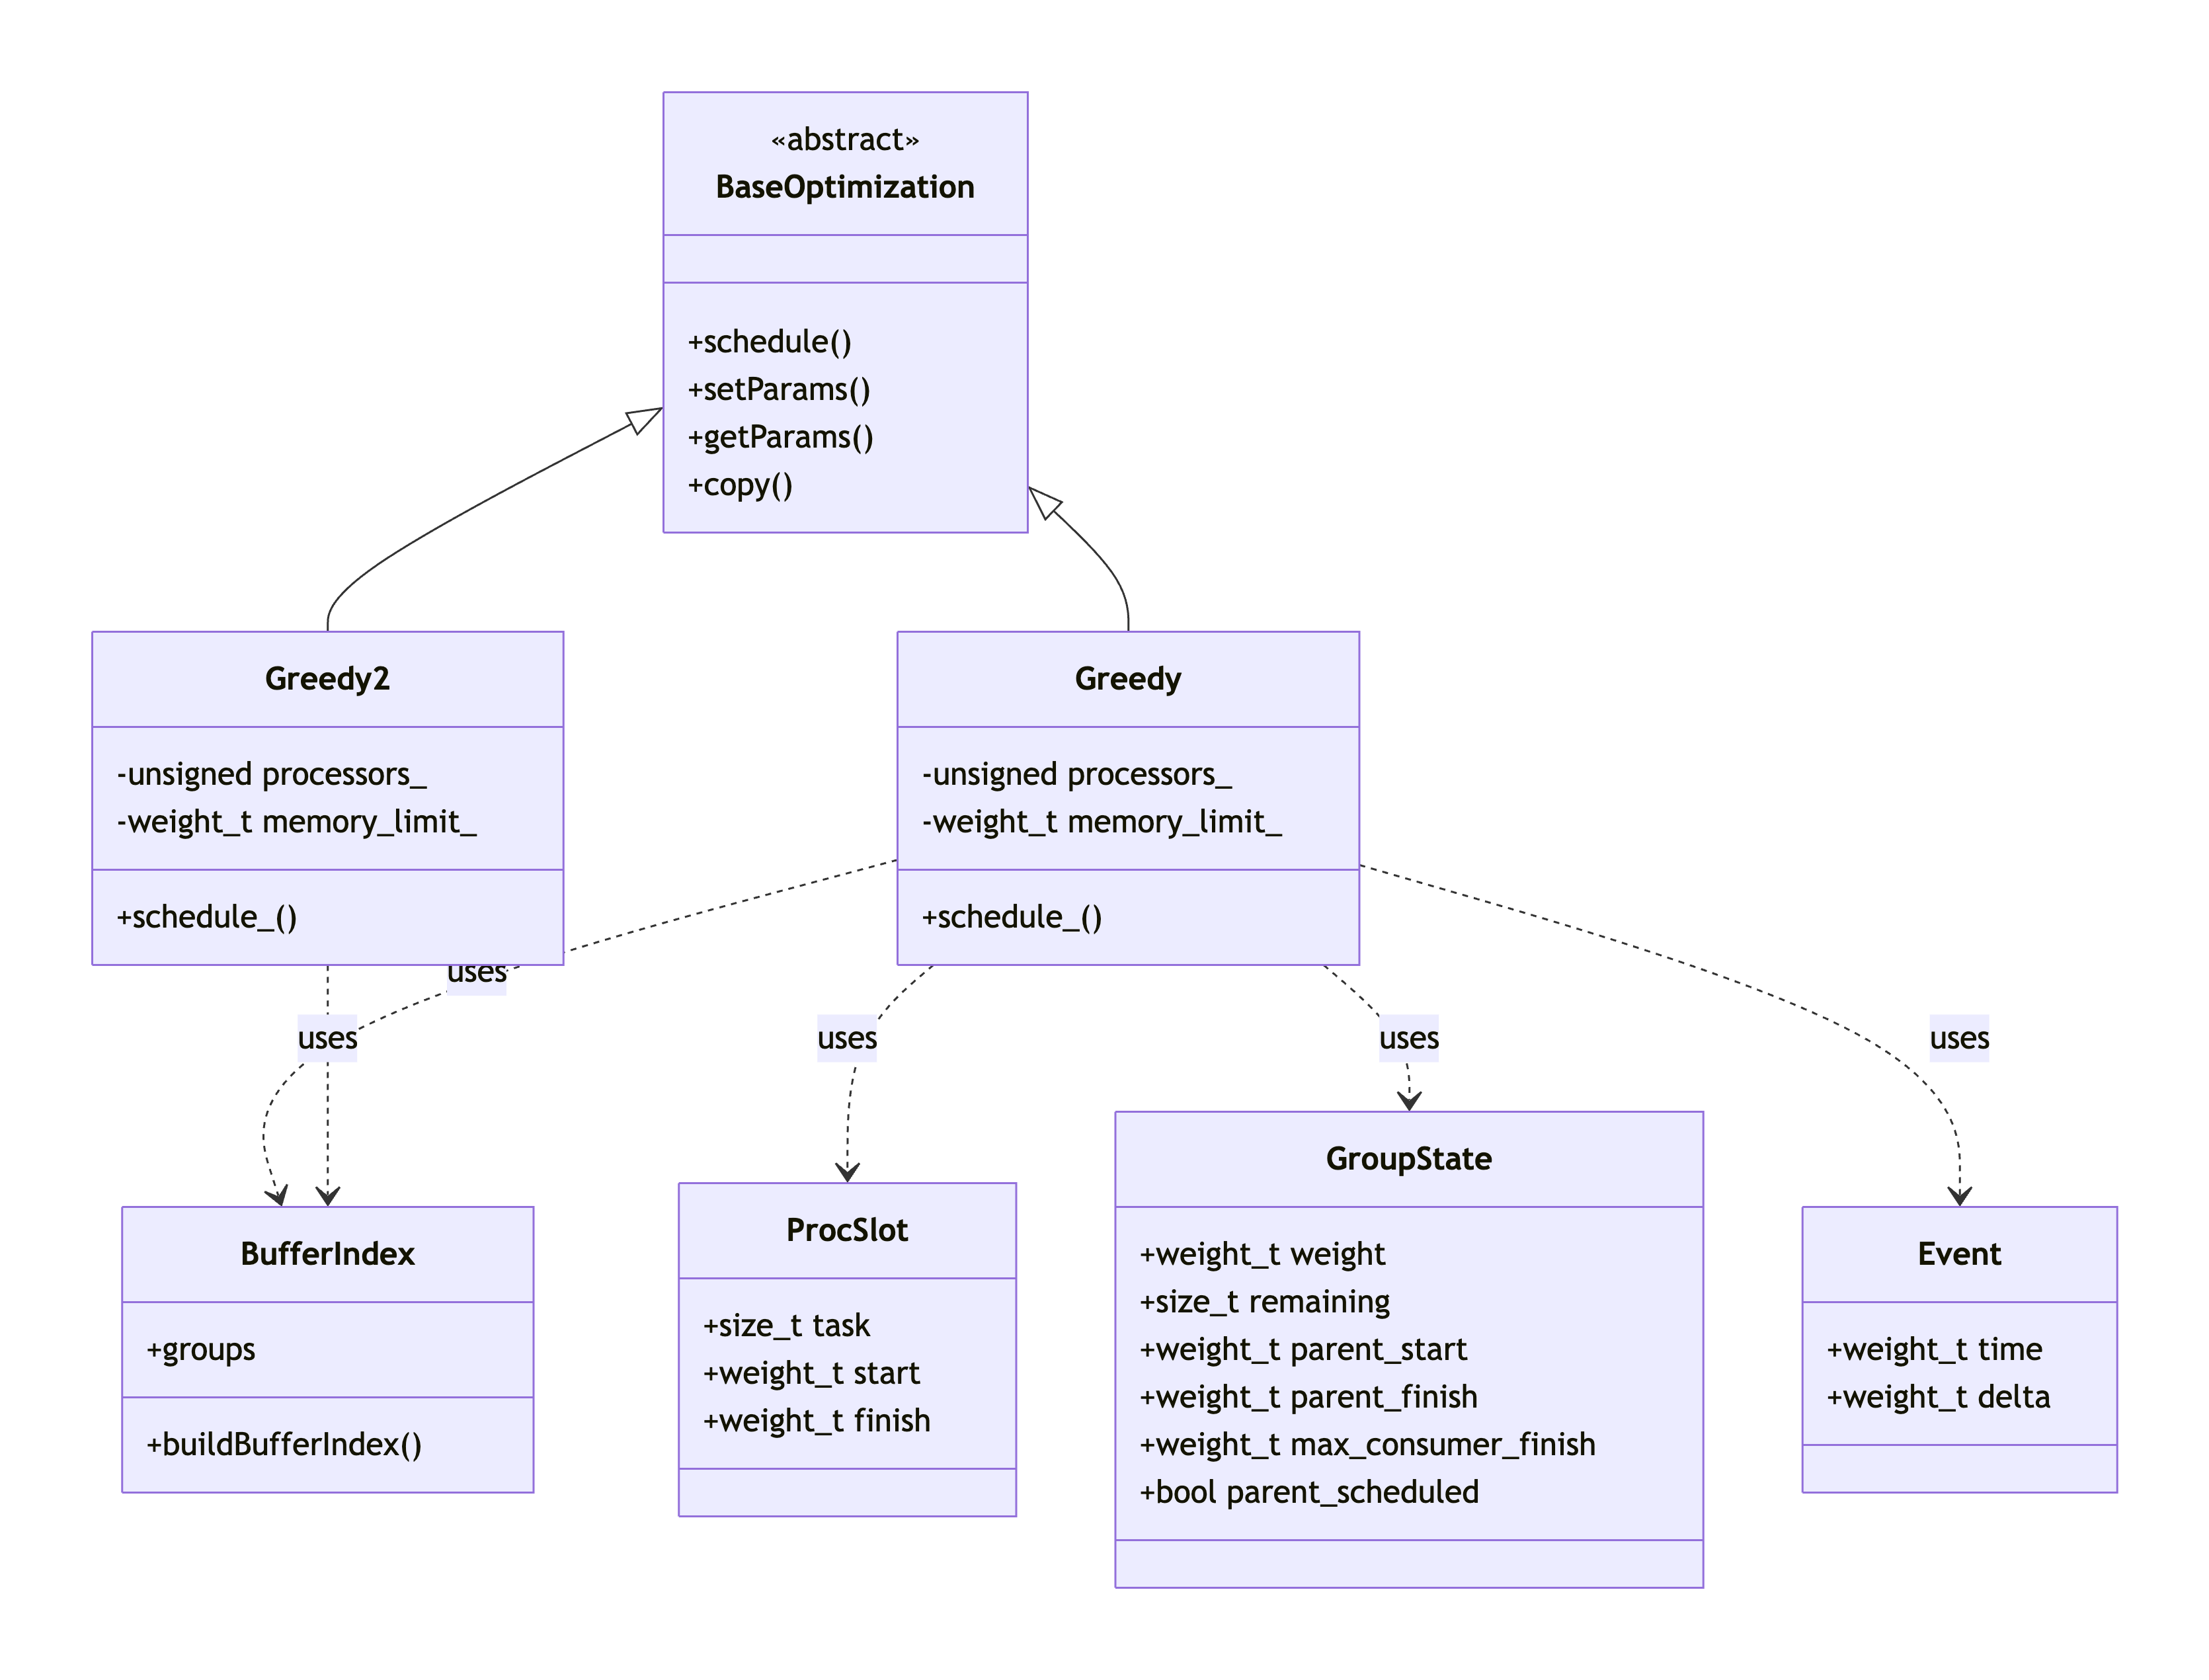
\includegraphics[width=1\textwidth]{pictures/greedy_class_diagram.png}
	\caption{Диаграмма классов жадного алгоритма}
	\label{fig:greedy_class_diagram}
\end{figure}

\paragraph{Базовый класс \texttt{BaseOptimization}}
Абстрактный класс, задающий интерфейс для всех алгоритмов оптимизации расписания. Содержит виртуальные методы \texttt{schedule()} (построение расписания), \texttt{setParams()}/\texttt{getParams()} (управление параметрами) и \texttt{copy()} (клонирование). Наследники должны реализовать конкретный метод \texttt{schedule\_()}.

\paragraph{Класс \texttt{Greedy} (EFT)}
Реализует жадный алгоритм, использующий эвристику \textbf{Earliest Finish Time (EFT)}. Ключевая функция — \texttt{earliestStartOnProcessor2()} — просматривает интервалы занятости процессора и находит подходящее окно.

\paragraph{Класс \texttt{Greedy2} (STS)}
Реализует эвристику \textbf{Smallest Time-Space (STS)}, учитывающую как длительность работы, так и её влияние на будущую занятость памяти. Вычисление оценки вынесено в отдельные переменные \texttt{output\_buffers\_weight\_sum} и \texttt{weighted\_duration\_sum} внутри основного цикла.

\paragraph{Вспомогательные структуры}
\begin{itemize}
	\item \texttt{ProcSlot} — описывает отрезок времени, занятый работой на процессоре (интервал $[start, finish)$).
	\item \texttt{GroupState} — состояние буфера: объём памяти, число оставшихся потребителей, время старта/завершения родительской работы и максимальное время завершения среди уже назначенных потребителей.
	\item \texttt{Event} — событие изменения занятости памяти (выделение или освобождение), используется при проверке допустимости по памяти.
	\item \texttt{BufferIndex} — индекс буферов, построенный по входному графу: для каждой работы хранит список её буферов, а для каждого буфера — список потребителей и объём. Используется для инициализации состояний \texttt{GroupState}.\\
\end{itemize}

\paragraph{Особенности реализации}
\begin{itemize}
	\item Все времена и объёмы памяти представлены целочисленным типом \texttt{weight\_t} (псевдоним \texttt{long long}).
	\item Процессоры нумеруются с 0 до $P-1$, расписание на каждом процессоре хранится как отсортированный вектор интервалов \texttt{ProcSlot}.
	\item Множество готовых работ поддерживается в \texttt{std::set} (автоматическая сортировка по идентификатору).
	\item Для ускорения поиска стартового окна на процессоре используется линейный проход по интервалам — в силу того, что число интервалов на процессор не превышает числа работ, а общее число работ редко превышает несколько тысяч, этого достаточно.
\end{itemize}

\subsection{Реализация подхода на базе ЦЛП}\label{sec:real_ILP}

Подход, описанный в разделе~\ref{sec:4_reduce_description}, реализован в виде набора скриптов на языке Python и Bash. Основные компоненты:

\begin{itemize}
	\item \texttt{make\_input\_times\_step2\_2.py} – транслятор, преобразующий входной граф работ в описание задачи ЦЛП на входном языке решателя SCIP (файл с расширением \texttt{.lp}).  
	Для каждого графа генерируется 10 упорядочений (см. подраздел~\ref{subsec:paral})
	Структура \texttt{.lp}-файла соответствует распределению, приведённому в табл.~\ref{tab:lp_sections}.
	
	\item \texttt{run\_many\_make\_inputs\_time\_for\_LP.py} – автоматизирует вызов транслятора для всех входных графов из каталога экспериментов. Из имени каждого файла извлекаются значения числа процессоров $P$ и лимита памяти $M$ (см. подраздел~\ref{subsec:datasets}), и эти параметры подставляются в глобальные переменные скрипта
	
	 \texttt{make\_input\_times\_step2\_2.py}.
	
	\item \texttt{run\_many\_solvers.py} – управляет выполнением серии экспериментов через обёрточный скрипт \texttt{run\_scip2.sh}. Ограничение времени работы решателя задаётся в файле \texttt{only\_time.set} (параметр \texttt{limits/time = 3600}).
	
	\item \texttt{run\_scip2.sh} – реализует параллельный запуск 8 экземпляров SCIP. Логи работы сохраняются в отдельные каталоги.
	
	\item \texttt{file\_reader\_and\_making\_json.py} – извлекает из логов SCIP значения переменных:
	\begin{itemize}
		\item $s_i$ (время старта работы $i$),
		\item $p_{ri}$ (номер процессора, назначенного работе $i$),
		\item вычисляет длительность как $\max_i (s_i + d_i)$.
	\end{itemize}
	Результат записывается в JSON-файл, полностью совместимый по структуре с выходными файлами жадных алгоритмов.\\\\\\
\end{itemize}

\begin{table}[ht]
	\centering
	\small
	\setlength{\tabcolsep}{4pt}
	\caption{Распределение переменных и ограничений по секциям \texttt{.lp}-файла}
	\label{tab:lp_sections}
	\begin{tabular}{|l|p{3cm}|p{6cm}|}
		\hline
		\textbf{Секция} & \textbf{Переменные / ограничения} & \textbf{Пояснение} \\
		\hline
		\texttt{Integer} & $l$, $s_i$, $\text{start}_{i,j}$, $\text{max\_end}_{i,j}$ & Целевая переменная, времена старта работ, начала и макс. завершения буферов \\
		\hline
		\texttt{Binary} & $m_{ij}$, $p_{ri}$, $t_{ij}$, $z_{ij}^{pq}$, $zz_{ij}^{pq}$, $a_{ij}^{pq}$, $aa_{ij}^{pq}$ & Отношения порядка, назначение на процессоры, пересечения буферов \\
		\hline
		\texttt{Subject to} & (\ref{eq:m_ge_frac})--(\ref{eq:m_le_frac}), (\ref{eq:prec}), (\ref{eq:no_conflict1})--(\ref{eq:no_conflict2}), (\ref{eq:z_start_new})--(\ref{eq:aa_end_new}) и др. & Основные линейные ограничения \\
		\hline
		\texttt{Bounds} & $m_{ii}=1$, $m_{ij}=1$ для $(i,j)\in E$ (включая транзитивные) & Фиксированные значения переменных предшествования \\
		\hline
		\texttt{Minimize} & $l$ & Целевая функция \\
		\hline
	\end{tabular}
\end{table}

Для генерации входных графов и подготовки наборов экспериментов использованы дополнительные скрипты:
\begin{itemize}
	\item \texttt{layered\_generator.py}, \texttt{random\_generator.py}, \texttt{triadag\_generator.py} – создают графы в «старом» формате (вершина, вес, список потомков) без учёта буферов.
	\item \texttt{converter.py} – преобразует «старые» графы в новый формат с буферами: назначает случайные длительности работ ($\in[10,100]$) и веса буферов ($\in[1,100]$), формирует два варианта группировки рёбер в буферы – один буфер (\texttt{\_1\_}) и равномерное корневое распределение (\texttt{\_N\_uniform\_}).
	\item \texttt{finding\_M\_and\_P.py} – для каждого полученного графа вычисляет на практике максимальное используемое число процессоров $P_{\max}$ и максимальную пиковую память $M_{\max}$ (при заведомо избыточных ресурсах). Затем создаёт 9 вариантов входных файлов ($3$ значения $P \times 3$ значения $M$) согласно сетке, описанной в подразделе~\ref{subsec:datasets}.
\end{itemize}

\subsection{Визуализатор временной диаграммы расписания}\label{sec:visual}

Для наглядного представления построенных расписаний (как полученных жадными алгоритмами, так и с помощью ЦЛП) разработан скрипт \texttt{gantt\_and\_memory.py} на языке Python с использованием библиотеки \texttt{matplotlib}. Он создаёт совмещённое изображение, состоящее из двух диаграмм:

\begin{enumerate}
	\item \textbf{Диаграмма Ганта} – отображает загрузку процессоров во времени. Каждая работа изображается цветным прямоугольником, внутри которого указан её идентификатор. По горизонтальной оси отложено время, по вертикальной – номера процессоров.
	\item \textbf{Диаграмма использования памяти} – показывает, как меняется суммарный объём занятой памяти в процессе выполнения расписания. По вертикальной оси отложен объём памяти, по горизонтальной – время. Дополнительно красной горизонтальной линией отмечается заданный лимит памяти $M$.
\end{enumerate}

\paragraph{Входные данные:}
\begin{itemize}
	\item JSON-файл с расписанием, содержащий для каждой работы номер процессора, время старта и завершения.
	\item Исходный TXT-файл графа работ в новом формате (с буферами), необходимый для определения, какие буферы активны в каждый момент времени.
\end{itemize}

\paragraph{Ключевые компоненты реализации:}
\begin{itemize}
	\item Функции рисования стрелок (\texttt{draw\_horiz\_arrow}, \texttt{draw\_vertical\_arrow},\\ \texttt{draw\_arc\_arrow}, \texttt{draw\_loop\_arrow} и др.) – используют \texttt{FancyArrowPatch} из\\ \texttt{matplotlib.patches}. Они проводят дуги и линии между работами, визуализируя зависимости по данным (рёбра графа). Тип стрелки зависит от взаимного расположения работ: горизонтальная, вертикальная, диагональная или дугообразная.
	\item Класс \texttt{ResourceVisualizer} – накапливает события изменения памяти (выделение и освобождение буферов) для каждого момента времени. Метод \texttt{visualize()} строит ступенчатую диаграмму, где каждый прямоугольник соответствует периоду активности конкретного буфера. Метод \texttt{add\_horizontal\_line()} добавляет линию заданного лимита памяти.
	\item Функция \texttt{get\_task\_coordinates} – вычисляет координаты работы на диаграмме Ганта по её времени старта, длительности и номеру процессора.
\end{itemize}

\paragraph{Выходные данные:}  
Скрипт отображает полученное изображение на экране (при интерактивном запуске) и может сохранить его в файл (например, в формате PNG) разрешением $300$ dpi.

Визуализатор активно используется при отладке алгоритмов, а также для качественного анализа полученных расписаний в ходе экспериментального исследования. С его помощью были построены, например, рисунки~\ref{fig:g6_greedy},~\ref{fig:g6_lp},~\ref{fig:EFT_20},~\ref{fig:lp_20}.

\subsection{Структура входного и выходного файлов}\label{sec:struct}

\subsubsection*{Входной файл (описание графа работ)}

Входной файл имеет расширение \texttt{.txt} и содержит строки в кодировке UTF-8.  
Первая строка является заголовком и содержит названия полей:
\begin{verbatim}
	id time weight_1: child_1 ... child_n, weight_2: child_1 ... child_n, ...
\end{verbatim}

Каждая последующая строка описывает одну работу (вершину графа) и имеет следующий формат:
\begin{verbatim}
	<id> <time> <буфер_1>, <буфер_2>, ..., <буфер_k>
\end{verbatim}
где
\begin{itemize}
	\item \texttt{<id>} — целочисленный идентификатор работы (от 0 до $n-1$);
	\item \texttt{<time>} — целочисленная длительность выполнения работы;
	\item \texttt{<буфер\_i>} имеет вид \texttt{<вес>: <список потомков>}, где \texttt{<вес>} — целое число, задающее объём памяти, занимаемый данным буфером, а \texttt{<список потомков>} — разделённые пробелами идентификаторы работ-потребителей этого буфера. Если у работы нет исходящих рёбер, в строке указывается единственный буфер \texttt{0:} (нулевой вес, пустой список потомков).
\end{itemize}

Буферы в строке разделяются запятой с пробелом (\texttt{`, `}). Внутри одного буфера после двоеточия может быть перечислено несколько потомков, что означает, что все они используют один и тот же буфер (и, следовательно, разделяют его данные). Пример строки для работы с двумя буферами:
\begin{verbatim}
	2   36   10: 3 6 7, 73: 4 8
\end{verbatim}
Это означает, что работа 2 длится 36 единиц времени, создаёт два буфера: первый весом 10 используется работами 3, 6, 7; второй весом 73 используется работами 4 и 8.

\subsubsection*{Выходной файл (расписание)}

Результат работы жадного алгоритма или решателя ЦЛП сохраняется в файл формата JSON с расширением \texttt{.json}. Файл содержит один объект, ключом которого является имя входного графа (без расширения), а значением — объект с полями, описывающими расписание. Структура JSON-объекта:

\begin{verbatim}
	{
		"имя_графа": {
			"makespan": целое,
			"runtime_sec": число с плавающей точкой,
			"size": целое,
			"schedule": {
				"id_вершины": {
					"processor": целое,
					"start": целое,
					"finish": целое
				},
				...
			}
		}
	}
\end{verbatim}

Поля означают:
\begin{itemize}
	\item \texttt{makespan} — общая длительность расписания (максимальное время завершения среди всех работ);
	\item \texttt{runtime\_sec} — реальное время работы алгоритма в секундах;
	\item \texttt{size} — число вершин в графе;
	\item \texttt{schedule} — словарь, где каждому идентификатору вершины соответствует словарь с тремя полями: \texttt{processor} — номер процессора (начиная с 0), на котором выполняется работа; \texttt{start} — время начала выполнения; \texttt{finish} — время завершения (\texttt{start} + длительность работы).
\end{itemize}
